\newpage
{\bfseries МРНТИ 20.23.15}

\sectionwithauthors{А.Ж. Танирбергенов, С.К. Серикбаева, Б.У. Бөбеева, Ш.Е. Ахметжанова, А.Д. Абдувалова}{ТАБИҒИ ТІЛДЕ ПАЙДАЛАНУШЫ ИНТЕРФЕЙСТЕРІН ҚҰРУ ӘДІСТЕРІ}

\begin{center}
{\bfseries \textsuperscript{1}А.Ж. Танирбергенов, \textsuperscript{1}С.К.
Серикбаева\textsuperscript{🖂}, \textsuperscript{2}Б.У. Бөбеева,
\textsuperscript{3}Ш.Е. Ахметжанова, \textsuperscript{3}А.Д. Абдувалова}

\textsuperscript{1}Л.Н.Гумилев атындағы Еуразия ұлттық университеті,
Астана қ., Қазақстан,

\textsuperscript{2}Орталық Азия Инновациялық Университеті, Шымкент,
Қазақстан,

\textsuperscript{3}М.Х.Дулати атындағы Тараз өңірлік университеті, Тараз
қ., Қазақстан
\end{center}
Корреспондент-автор:  \emph{inf\_8585@mail.ru}



Қазіргі заманғы технологиялық даму жағдайында пайдаланушы интерфейстері
адамның компью-терлік бағдарламалармен немесе құрылғылармен өзара
әрекеттесуінде маңызды рөл атқарады, бұл олардың қарапайымдылығы,
тиімділігі және жалпы пайдаланушы тәжірибесін анықтайды. NLP UI идеясы
табиғи тілді өңдеу (NLP), машиналық оқыту және жасанды интеллект
алгоритмдерін қолдану-ға негізделген. Зерттеу барысында осындай
интерфейстерді құру әдістері, олардың артықшылықтары мен шектеулері,
сонымен қатар оларды одан әрі дамыту перспективалары талқыланды. ТТИ
платфор-маларын талдау, мысалы, Google Dialogflow, Microsoft Bot
Framework, Wit.ai, IBM Watson Assistant және Amazon Lex, пайдаланушыға
ыңғайлы интерфейстерді дамытуда маңызды рөл атқарады. Әдіс-тер мен
материалдар бөлімінде табиғи тілде пайдаланушы интерфейстерін жасауға
арналған қолда-ныстағы әдістер, соның ішінде сөйлеуді тану және синтездеу
жүйелері, машиналық оқыту алгоритм-дері және морфологиялық, синтаксистік
және семантикалық талдау талқыланады. Бұл тәсілдер пай-даланушы
сұраныстарын тереңірек түсінуге және дәлірек жауаптар беруге мүмкіндік
береді.

{\bfseries Түйінді сөздер:} табиғи тіл, интерфейс, табиғи тілді өңдеу
(NLP), семантика, сұраныс.


\sectionheading{МЕТОДЫ СОЗДАНИЯ ПОЛЬЗОВАТЕЛЬСКИХ ИНТЕРФЕЙСОВ НА ЕСТЕСТВЕННОМ ЯЗЫКЕ}

\begin{center}

{\bfseries \textsuperscript{1}А.Ж. Танирбергенов, \textsuperscript{1}С.К.
Серикбаева\textsuperscript{🖂}, \textsuperscript{2}Б.У. Бөбеева,
\textsuperscript{3}Ш.Е. Ахметжанова,\textsuperscript{3}А.Д. Абдувалова}

\textsuperscript{1}Евразийский национальный университет имени
Л.Н.Гумилева, Астана, Казахстан \textsuperscript{2}Центрально-Азиатский
инновационный университет, Шымкент, Казахстан \\ \textsuperscript{3}Таразский региональный университет им.М. Х. Дулати,
Тараз, Казахстан

e-mail:inf\_8585@mail.ru
\end{center}

В данной работе рассматриваются методы и технологии создания
пользовательских интерфейсов на естественном языке. В условиях
современного технологического развития пользовательские ин-терфейсы
играют важную роль во взаимодействии человека с компьютерными
программами и ус-тройствами, что определяет их простоту, эффективность и
общий пользовательский опыт. Идея пользовательского интерфейса на основе
NLP основана на использовании алгоритмов обработки естественного языка
(NLP), машинного обучения и искусственного интеллекта. В ходе
исследования обсуждались методы создания таких интерфейсов, их
преимущества и ограничения, а также перспек-тивы дальнейшего развития.
Анализ платформ TTI, таких как Google Dialogflow, Microsoft Bot
\\Framework, Wit.ai, IBM Watson Assistant и Amazon Lex, показал их важную
роль в разработке удобных интерфейсов. В разделе "Методы и материалы"
обсуждаются существующие методы создания поль-зовательских интерфейсов на
естественном языке, включая системы распознавания и синтеза речи,
алгоритмы машинного обучения, а также морфологический, синтаксический и
семантический анализ. Эти подходы позволяют глубже понять запросы
пользователей и давать более точные ответы.

{\bfseries Ключевые слова:} естественный язык, интерфейс, обработка
естественного языка (NLP), семан-тика, запрос.

\sectionheading{METHODS FOR CREATING USER INTERFACES IN NATURAL LANGUAGE}
\begin{center}
{\bfseries \textsuperscript{1}А. Tanirbergenov, \textsuperscript{1}S.
Serikbayeva\textsuperscript{🖂}, \textsuperscript{2}B. Bobeeva,
\textsuperscript{3}Sh. Akhmetzhanova,{3}A. Abduvalova}

\textsuperscript{1}L.N. Gumilyov Eurasian National University,Department
of Information Systems, Astana, Kazakhstan

Central Asian Innovation University, Shymkent, Kazakhstan

\textsuperscript{3}Taraz Regional University named after M.KH.Dulaty,
Taraz, Kazakhstan

e-mail: inf\_8585@mail.ru
\end{center}

This paper discusses methods and technologies for creating user
interfaces in natural language. In the context of modern technological
development, user interfaces play an important role in human interaction
with computer programs and devices, which determines their simplicity,
efficiency and overall user expe-rience. The idea of an NLP-based user
interface is based on the use of natural language processing (NLP)
algorithms, machine learning and artificial intelligence. The research
discussed methods for creating such interfaces, their advantages and
limitations, as well as prospects for further development. Analysis of
TTI platforms such as Google Dialogflow, Microsoft Bot Framework, Wit.ai
, IBM Watson Assistant and Amazon Lex, showed their important role in
the development of user-friendly interfaces. The Methods and Materials
section discusses existing methods for creating user interfaces in
natural language, including speech recognition and synthesis systems,
machine learning algorithms, as well as morphological, syntactic and
semantic analysis. These approaches allow for a deeper understanding of
user requests and provide more accurate answers.

{\bfseries Keywords:} natural language, interface, natural language
processing (NLP), semantics, query.

\begin{multicols}{2}
{\bfseries Кіріспе.} Технологияны дамытудың қазіргі әлемінде пайдаланушы
интерфейстері адамның компьютерлік бағдарламамен немесе құрылғымен өзара
әрекеттесуінде шешуші рөл атқарады. Олар пайдаланудың қарапайымдылығын,
жұмыс тиімділігін және жалпы пайдаланушы тәжірибесін анықтайды. Осы
саладағы елеулі жетістіктерге қарамастан, ыңғайлы және интуитивті
пайдаланушы интерфейстерін құру әзірлеушілер үшін қиын болып қала
береді.

Бұл мәселені шешудің инновациялық тәсілдерінің бірі-табиғи тілде
пайдаланушы интерфейстерін құру әдісі (natural language UI, NLP UI). Бұл
әдіс пайдаланушыларға басқа адаммен сөйлесу сияқты табиғи тілді қолдана
отырып, бағдарламалық жасақтамамен немесе құрылғымен өзара әрекеттесуге
мүмкіндік береді. Бұл тәсіл интуитивті және икемді өзара әрекеттесудің
жаңа мүмкіндіктерін ашады.

Табиғи тілде пайдаланушы интерфейстерін құру идеясы табиғи тілді өңдеу
алгоритмдерін (Natural Language Processing, NLP), машиналық оқытуды және
жасанды интеллектті қолдануға негізделген. Бұл технологиялар жүйелерге
табиғи тілді түсінуге және түсіндіруге, сондай-ақ тиісті жауаптар мен
командаларды құруға мүмкіндік береді {[}1{]}.

NLP UI артықшылықтары айқын: бұл құрылғылар мен бағдарламалық
жасақтаманың өзара әрекеттесуін пайдаланушылар үшін табиғи және
интуитивті етеді, бұл оқу уақытын қысқартады және пайдалану тиімділігін
арттырады. Осының арқасында пайдаланушылар жаңа өнімдер мен қызметтерді
тезірек игере алады, сонымен қатар күнделікті тапсырмаларды тиімдірек
орындай алады.

Дегенмен, оның артықшылықтарына қарамас-тан, табиғи тілде пайдаланушы
интерфейстерін жасау да өзінің қиындықтары мен шектеулеріне тап болады.
Олардың бірі-пайдаланушы сұраныстарын дәл түсінудің қиындығы, әсіресе
тілдің түсініксіз немесе күрделі конструкциялары жағдайында.

Дегенмен, технологияның дамуымен және жаңа NLP әдістері мен
алгоритмдерінің пайда болуымен бұл мәселелер біртіндеп азайып, табиғи
тілдегі пайдаланушы интерфейстерін барған сайын танымал және қолжетімді
етеді. Бұл зерттеуде біз осындай интерфейстерді құрудың әртүрлі
әдістерін, олардың артықшылық-тары мен шектеулерін және оларды одан әрі
дамыту перспективаларын қарастырамыз.

Табиғи тілдік интерфейстерді (ТТИ) құру платформаларын талдау табиғи
тілді өңдеу саласын дамытудағы маңызды қадам болып табылады (Natural
Language Processing, NLP). Бұл платформалар әзірлеушілерге техникалық
мәліметтерді терең түсінбестен мәтін мен сөйлеуді өңдеу мүмкіндіктерін
қолданбалар мен қызметтерге біріктіруге мүмкіндік береді.

Бірінші назар аударарлық платформа - Google-дің Dialogflow. Ол
чатботтарды, виртуалды көмекшілерді және басқа да ТТИ -ді құрудың кең
функционалдығын ұсынады. Dialogflow мәтінді талдаудың, интенттер мен
контекстті анықтаудың және басқа Google қызметтерімен интеграциялаудың
қуатты құралдарына ие {[}2{]}.

Тағы бір маңызды платформа-Microsoft Bot Framework. Бұл мәтіндік ғана
емес, сонымен қатар дауыстық интерфейстерді де қолдайтын чат-боттарды
әзірлеуге арналған құралдар жиынтығы. Azure интеграциясының арқасында
Bot Framework Машиналық оқыту модельдерінің ауқымдылығы мен оқу
мүмкіндіктерін ұсынады.

Wit.ai Facebook-тен-ТТИ -ді дамытуға арналған тағы бір танымал
платформа. Ол қолданудың қарапайымдылығымен және әртүрлі тілдерді жақсы
қолдауымен танымал. Wit.ai мәтін мен аудионы өңдеуге арналған API,
сондай-ақ өз модельдеріңізді құруға және үйретуге арналған құралдарды
ұсынады.

IBM Watson Assistant-бұл ТТИ құрудың тағы бір қуатты құралы. Ол интентті
тану, мәтіннің тоналдылығын талдау және әртүрлі байланыс арналарымен
интегрциялау сияқты көптеген мүмкіндіктерді ұсынады. Watson Assistant
сонымен қатар көмекшілерді масштабтау және жекелендіру мүмкіндіктерін
ұсынады.

Amazon Lex-Amazon Web Services компаниясы-ның табиғи тілді өңдеу қызметі.
Ол сөйлеуді тану және синтездеу мүмкіндіктерін, сондай-ақ басқа AWS
қызметтерімен интеграцияны қамтамасыз етеді. Amazon Lex дайын модельдер
мен машиналық оқыту құралдарын қолдана отырып, жоғары деңгейлі ТТИ
құруға мүмкіндік береді.

Табиғи тілде пайдаланушы интерфейстерін құруда адам мен компьютерлік
жүйенің тиімді өзара әрекеттесуін анықтайтын іргелі теориялық принциптер
бар. Бұл принциптерге лингвистикалық негіздер, өзара әрекеттесу
психологиясы, интерфейс дизайны, табиғи тілді өңдеу технологиялары
(NLP), Машиналық оқыту және интерфейс психологиясы кіреді.

Лингвистикалық принциптер сәйкес сөздер мен сөз тіркестерін таңдауға,
мәтінді құрылымдауға және пайдаланушылардың сұраныстарын дұрыс
түсіндіруге мүмкіндік береді. Өзара әрекеттесу психологиясы ақпаратты
қабылдау, шешім қабылдау және кері байланысқа жауап беру ерекшеліктерін
ескеруге көмектеседі. Интерфейс дизайны ыңғайлы және тартымды
интерфейстерді құруға ықпал ететін ақпараттың визуалды ұйымдастырылуын
анықтайды {[}3{]}.

Табиғи тілді өңдеу технологиялары (NLP) табиғи тілдегі мәтінді талдауды,
түсінуді және генерациялауды қамтамасыз етуде маңызды рөл атқарады.
Машиналық оқыту және жасанды интеллект интерфейстерге пайдаланушы
тәжірибесі негізінде жұмысын жақсартуға мүмкіндік береді. Интерфейс
психологиясы адамдардың интерфейстермен қалай әрекеттесетінін түсінуге
көмектеседі және оларды оңтайландыру принциптерін ұсынады. Осы теориялық
негіздердің барлығы пайдаланушылардың қажеттіліктеріне сәйкес келетін
және пайдаланудың ыңғайлылығы мен тиімділігін қамтамасыз ететін табиғи
тілде пайдаланушы интерфейстерін құруды қамтамасыз ету арқылы өзара
әрекеттеседі.

Іс жүзінде осы теориялық принциптерді қолдану кешенді тәсілді және нақты
жағдайды мұқият талдауды қажет етеді. Бұл талдау мақсатты аудиторияның
ерекшеліктерін, олардың қажеттіліктерін, жүйені пайдалану мәнмәтінін,
сондай-ақ техникалық шектеулер мен мүмкіндіктерді зерттеуді
қамтиды.Келесі қадам-интерфейстің прототиптерін жасау және
пайдаланушылардың қатысуымен тестілеу. Бұл пайдаланушылардың нақты
қажеттіліктері мен қалауларын ескере отырып, кері байланыс алуға және
интерфейстің дизайны мен функционалдығына түзетулер енгізуге мүмкіндік
береді. Алынған кері байланыс пен пайдалану ортасындағы өзгерістер
негізінде интерфейсті үнемі жетілдіру және жаңарту оның өзектілігі мен
тиімділігін сақтаудың негізгі аспектісі болып табылады {[}4{]}.
Осылайша, табиғи тілде пайдаланушы интерфейстерін құрудың теориялық
негіздері пайдаланушы тәжірибесін жақсартуға және мақсаттарға жетуге
ықпал ететін ыңғайлы, интуитивті және тиімді жүйелерді әзірлеу бойынша
практикалық жұмыстың негізін құрайды.

Пайдаланушы интерфейстеріндегі табиғи тіл ұғымы адам мен компьютерлік
жүйенің өзара әрекеттесуінің ыңғайлылығы мен тиімділігін қамтамасыз
етуде шешуші рөл атқарады. Бұл контекстегі табиғи тіл пайдаланушылардың
өз ойлары мен сұрауларын арнайы командаларды немесе техникалық
терминдерді үйренуді қажет етпестен, әдеттегі әңгімедегідей жеткізе білу
қабілетін білдіреді. Табиғи тілді пайдалану техникалық дайындық
деңгейіне қарамастан, пайдаланушылардың кең ауқымы үшін интуитивті
интерфейстер жасауға мүмкіндік береді. Мұндай интерфейстер табиғи және
ыңғайлы өзара әрекеттесуді қамтамасыз етеді, кіру шегін азайтады және
оқу процесін жылдамдатады.

Пайдаланушы интерфейстерінде табиғи тілді қолданудың бір мысалы-Apple,
Google Assistant және Amazon Alexa Siri сияқты виртуалды көмекшілер. Бұл
жүйелер пайдаланушыларға табиғи тілді қолдана отырып, сұрақтар қоюға
және дауыспен командалар беруге мүмкіндік береді, бұл өзара әрекеттесу
процесін табиғи және ыңғайлы етеді.

Пайдаланушы интерфейстерінде табиғи тіл ұғымын одан әрі дамыту Машиналық
оқыту және табиғи тілді өңдеу (Natural Language Processing, NLP)
технологияларымен интеграцияны қамтиды. Бұл жүйелерге сұраныстардың
мәнмәтінін түсінуге, тілдің нюанстарын ескеруге және тіпті
пайдаланушылардың кері байланысы негізінде қабілеттерін жақсартуға
мүмкіндік береді.

Қазіргі заманғы қосымшалар мен құрылғылар-да табиғи тілді талдау
негізінде жұмыс істейтін автотолтыру және автоматты түзету функциялары
жиі кездеседі. Бұл теруді жылдам әрі ыңғайлы етеді, қателіктер
ықтималдығын азайтады.

Табиғи тіл сонымен қатар Ақылды үйді басқаруға арналған интерфейстер
саласында маңызды рөл атқарады, мұнда пайдаланушылар өз құрылғыларын
табиғи тілдегі қарапайым командаларды қолдана отырып басқара алады, бұл
өмірді ыңғайлы және тиімді етеді.

Бұл тұжырымдаманың болашақ дамуы сөйлеуді тану мен контекстті түсінудің
одан да жетілдірілген технологияларын қамтуы мүмкін, бұл пайдаланушы
интерфейстеріндегі адам мен компьютерлік жүйе арасындағы одан да табиғи
және икемді өзара әрекеттесуге әкеледі.

Пайдаланушы интерфейстеріндегі табиғи тіл (Natural Language in User
Interfaces) -- бұл пайдаланушыға орыс немесе ағылшын сияқты қарапайым
адам тілін қолдана отырып, компьютерлік жүйемен немесе қосымшамен өзара
әрекеттесу мүмкіндігін беру тәсілі. Бұл интерфейсті түсінікті, қол
жетімді және пайдаланушыларға ыңғайлы етеді, өйткені олар белгілі бір
командаларды немесе интерфейс элементтерін есте сақтаудың қажеті жоқ.

Пайдаланушы интерфейстерінде табиғи тілді қолдану сөйлеуді тану және
синтездеу функцияларын, мәтінді өңдеуді, семантиканы талдауды және т.б.
қамтуы мүмкін {[}5{]}. Бұл пайдаланушыларға жүйе автоматты түрде
түсіндіретін және өңдейтін өз тілін пайдаланып сұрақтар қоюға,
командалар беруге немесе ақпарат сұрауға мүмкіндік береді.

Бұл тәсіл құрылғылармен және қосымшалар-мен өзара әрекеттесуді едәуір
жеңілдетеді, әсіресе техникалық интерфейстермен тәжірибесі жоқ немесе
белгілі бір командаларды үйренуге уақыт жұмсағысы келмейтін
пайдаланушылар үшін. Сондықтан әзірлеушілер ыңғайлы және интуитивті
пайдаланушы интерфейстерін жасау үшін әртүрлі табиғи тіл технологияларын
белсенді түрде зерттейді және енгізеді.

Пайдаланушы интерфейстеріндегі табиғи тілдің көптеген артықшылықтары
бар. Ең бастысы-интерфейстің қол жетімділігі мен ыңғайлылығын жақсарту
{[}6{]}. Пайдаланушыларға құрылғымен немесе қосымшамен өзара әрекеттесу
оңайырақ және ыңғайлы болады, өйткені олар күрделі командаларды немесе
интерфейс функционалдығын есте сақтаудың қажеті жоқ.

Сонымен қатар, табиғи тілді қолдану интуитивті және жекелендірілген
өзара әрекеттесуге мүмкіндік береді. Пайдаланушылар өздерінің
сұраныстары мен тілектерін табиғи стильде білдіре алады, бұл пайдалану
тәжірибесін жағымды және тиімді етеді.

Табиғи тілді өңдеу технологиялары үнемі дамып келеді және күн өткен
сайын дәлірек және жетілдіріліп отырады. Бұл Пайдаланушының тілін
түсініп қана қоймай, оның қалауы мен мінез-құлқына бейімделе алатын
ақылды интерфейстерді құрудың жаңа мүмкіндіктерін ашады.

Тұтастай алғанда, пайдаланушы интерфейсте-рінде табиғи тілді пайдалану
технологияны пайдаланушылардың барлық санаттары үшін мейірімді және
қолжетімді етуге көмектеседі, бұл әртүрлі құрылғылар мен қолданбалардың
қанағаттану деңгейі мен тиімділігіне ықпал етеді.

{\bfseries Материалдар мен әдістер.} Табиғи тілде пайдаланушы
интерфейстерін жасау (Natural Language User Interfaces, NLU) қазіргі
ақпараттық технологиялар әлемінде барған сайын танымал бола түсуде. Бұл
компьютерлік жүйелермен өзара әрекеттесудің ыңғайлы және интуитивті
тәсілдеріне қажеттіліктің артуына байланысты. Осы саладағы қолданыстағы
әдістер мен технологияларды шолу қазіргі даму жағдайын және одан әрі
даму бағыттарын түсінуге мүмкіндік береді.

Табиғи тілде пайдаланушы интерфейстерін құрудың негізгі әдістерінің бірі
табиғи тілді өңдеу (NLP) технологияларын пайдалану болып табылады. Бұл
технологиялар компьютерлерге табиғи тілді түсінуге және талдауға
мүмкіндік береді, олар пайдаланушылармен адамдар сияқты әрекеттесе
алатын интерфейстер жасауға мүмкіндік береді {[}7{]}.

Қолданыстағы әдістер мен технологиялардың ішінде пайдаланушыларға
дауыстық командалар мен сұраныстарды пайдалана отырып, компьютермен
өзара әрекеттесуге мүмкіндік беретін сөйлеуді тану және синтездеу
жүйелері ерекшеленеді. Мұндай жүйелер пайдаланушыларға ыңғайлы болу үшін
дауыстық көмекшілерде, мобильді құрылғыларда және басқа қолданбаларда
белсенді қолданылады.

Табиғи тілдегі пайдаланушы интерфейстерін құрудың тағы бір маңызды
аспектісі машиналық оқыту алгоритмдерін әзірлеу және пайдалану болып
табылады. Бұл алгоритмдер интерфейстер-ді тиімдірек және пайдалануды
жеңілдете отырып, пайдаланушының әртүрлі байланыс мәнерлері мен
сипаттамаларына бейімделе алатын үлгілерді жасауға мүмкіндік береді.

Табиғи тілде пайдаланушы интерфейстерін құру саласындағы елеулі
жетістіктерге қарамастан, одан әрі зерттеу мен дамытуды талап ететін
көптеген қиындықтар мен мәселелер әлі де бар {[}8{]}. Оларға сөйлеуді
тану дәлдігін жақсарту, контекстті түсінуді жақсарту және компьютерлік
жүйелермен бай қарым-қатынас жасау үшін басқа технологиялармен біріктіру
кіреді.

Интерфейс пайдаланушының өзара әрекеттесуі-нің ыңғайлылығы мен
тиімділігін қамтамасыз етуге арналған кез келген бағдарламалық жүйенің
ажырамас бөлігі болып табылады. Ол соңғы пайдаланушыға бағытталған және
бағдарлама туралы жалпы әсерді қалыптастыруда негізгі рөл атқарады.
Көбінесе пайдаланушы интерфейстің ыңғайлылығы мен анықтығына негізделген
қолданбаны пайдалануды шешеді.

Интерфейсті әзірлеу -- пайдаланушының қажеттіліктерін мұқият талдауды
және түсінуді талап ететін күрделі және көп уақытты қажет ететін
процесс. Сарапшылардың пікірінше, интерфейсті жобалау және әзірлеу
жобаны жүзеге асыруға кететін уақыттың жартысынан көбін құрайды {[}9{]}.

Интерфейстің функционалдық аспектілерін ғана емес, сонымен қатар оның
эстетикалық дизайнын, визуалды әсерін және ыңғайлылығын да ескеру
маңызды. Идеал интерфейс интуитивті, шарлау оңай және мақсатты
аудиторияның қажеттіліктерін қанағаттандыруы керек. Бағдарламаның әсері
және оның нарықта сәтті жүзеге асуы пайдаланушы интерфейсінің қаншалықты
жақсы құрастырылғанына байланысты.

Пайдаланушы интерфейсін анықтаудың бірнеше негізгі жолдары бар:

1. Тіл спецификациясы: Бұл жағдайда интерфейстің синтаксисін анықтау
үшін арнайы тілдер қолданылады. Бұл тілдер декларативті, объектіге
бағытталған, оқиғаға негізделген және т.б.

2. Графикалық спецификация: визуалды бағдарламалау, демонстрациялар және
үлгілер арқылы интерфейсті анықтаумен айналысады. Бұл әдіс әдетте
интерфейстердің шектеулі жиынтығын қолдайды.

3. Объектіге бағытталған тәсілге негізделген спецификация: Объектілерді
тікелей манипуля-циялау принципіне негізделген. Пайдаланушы өңдеушілер,
мәзірлер, диалогтық терезелер және түймелер сияқты жеке нысандармен
әрекеттеседі.

4. Қолданбалы тапсырманың семантикасына негізделген интерфейс
спецификациясы: Интерфейс қолданбалы тапсырманың семантика-сының
спецификациясы негізінде автоматты түрде жасалады. Дегенмен, интерфейсті
сипаттаудың күрделілігі дамуды бәсеңдетуі мүмкін.

Бүгінгі күні оларды жүзеге асырудың әртүрлі әдістерін қолдайтын
интерфейстерді әзірлеуге арналған көптеген құралдар бар {[}10{]}. Олар
бар үлгілер мен параметрленген құрамдастарды пайдалану арқылы жаңа
интерфейстерді жасауды жеңілдетеді.

Графикалық пайдаланушы интерфейстерін жылдам және сапалы әзірлеуге
арналған ең кең тараған пакет Motif болып табылады. Солтүстік Американың
OSF консорциумында әзірленген бұл пакет Xt Intrinsics идеяларының дамуы
болып табылады.

Табиғи тілді өңдеудің әртүрлі тәсілдері бар. Алғашқы тәсілдердің бірі
сөйлемге синтаксистік талдау жасауға негізделген. Бұл кезеңде сөйлем
ішіндегі синтаксистік байланыстар анықталып, сөйлемнің түрі, құрылымы
анықталады. Ол үшін талданатын тілге байланысты арнайы лексикалық және
синтаксистік ережелер қолданылады.

Сөйлемді талдау процесі тізбектей және бірнеше кезеңмен жүзеге
асырылады. Ол морфологиялық және морфемиялық талдау кезеңдерін
қадағалайды. Бұл кезеңде әрбір сөздің басқа сөйлем мүшелерімен байланысы
алынады, бұл грамматикалық категориялардың мағыналарын анықтауға
мүмкіндік береді.

Морфологиялық талдау синтаксистік талдаудың алдында тұрады және әрбір
сөздің сөйлем мүшесі, септелуі, регистр және басқалары сияқты
морфологиялық белгілерін анықтауға мүмкіндік береді. Бұл белгілер
сөйлемнің синтаксистік құрылымын анықтауда шешуші рөл атқарады {[}11{]}.

Морфологиялық сипаттамалардың саны мен әртүрлілігі нақты тілге
байланысты өзгеруі мүмкін, бұл талдау процесіне де әсер етеді.

Орыс тіліндегі табиғи тілді морфологиялық талдау үшін әртүрлі тәсілдер,
соның ішінде ықтималдық көзқарас, «бұлдыр» және «қытырлақ» морфология
қолданылады. Дегенмен, бұл процесте ең көп таралған тәсіл «айқын»
морфологияны қолдануға негізделген.

«Айқын» тәсіл орыс сөздерінің негізгі флекстік формаларын және олардың
сәйкес кодтарын қамтитын «Зализняк» сөздігі сияқты грамматикалық
сөздікке сүйенеді. Бұл сөздік ережелерге негізделген сөздің барлық
мүмкін формаларын көрсетуге мүмкіндік береді. Морфологиялық талдау
талданатын сөздің морфологиялық белгілерін анықтау үшін осы сөз
формалары мен олардың кодтарын пайдаланады.

Зализняктың грамматикалық сөздігіне негізделген сөздікті құру процесі
әрқайсысы үшін сөз формаларының жиынтығы жасалған барлық сөздерді
санаудан басталады. Бұл сөз формалары кейіннен морфологиялық талдауда
қолдану үшін сөздікке енгізіледі. Осылайша, бұл сөздік талданатын сөздің
морфологиялық сипаттамасын береді {[}12{]}.

Бұл табиғи тілді өңдеу әдісі сөздердің морфологиялық ерекшеліктерін дәл
анықтауға мүмкіндік береді, бұл орыс тіліндегі мәтіндерді талдау кезінде
маңызды қадам болып табылады.

Орыс тілінің морфемиялық талдауы әрбір сөзді префикс, жалғау, түбір,
жұрнақ және түбір сияқты құрамдас бөліктерге бөлуге мүмкіндік береді.
Бұл сөздің құрылымын және оның грамматикалық ерекшеліктерін түсінуге
көмектесетін мәтінді өңдеудің маңызды кезеңі.

Дегенмен, орыс тіліндегі морфемалардың сөздігі, әдетте, сөзде қандай
морфемалар бар екендігі туралы ақпарат береді, бірақ әрбір морфеманың
түрін көрсетпейді. Мысалы, сөздің қай бөлігі префикс, қайсысы түбір
екенін көрсетпейді. Бұл сөздің құрылымын морфемалық сөздіктегі
мәліметтерге сүйене отырып, біржақты анықтауға болмайтынын білдіреді
{[}13{]}.

Бұл ретте орыс сөзіндегі морфемалар тізбегі әдетте қатаң түрде
анықталады. Сөз префикстен, содан кейін түбірден басталып, жұрнақ пен
жалғаумен аяқталады. Алайда бұл бөліктердің кейбірі сөзде жоқ болуы
мүмкін.

Морфемалық сөздікте жоқ сөзді талдау үшін орыс тіліндегі морфемалардың
стандартты тізбегін, сондай-ақ мағыналарының ауыспалылы-ғымен шектелетін
мүмкін префикстер, жұрнақтар және жалғаулардың тізімін пайдалануға
болады. Бұл сөзді талдауға және морфемалық сөздіктегі анық мәліметтерсіз
де оның құрылымын анықтауға мүмкіндік береді.

Сонымен, орыс тілінің морфематикалық талдауы құрылымды түсінудің маңызды
құралы болып табылады.

Табиғи тілдегі пайдаланушы сұранысын өңдеу әдісінің шамамен диаграммасы:

1. Морфологиялық талдау:

\hspace{0.5cm}- Сұрауды жеке сөздерге талдау.

\hspace{0.5cm}- Әр сөздің сөйлем мүшесі, септелуі, регистр және басқалары сияқты
морфологиялық белгілерін анықтау.

2. Талдау:

\begin{itemize}
  \setlength{\itemindent}{1cm} 
\item
  Сөйлемдегі сөздер арасындағы синтаксис-тік байланыстарды анықтау.
\item
  Сөйлемнің бас және басыңқы мүшелерін анықтау.
\item
  Ұсыныс түрін анықтау.
\end{itemize}

3. Семантикалық талдау:

\hspace{0.5cm}- Сұраныстың мағынасын және оның мазмұнын талдау.

\hspace{0.5cm}- Өтініште көрсетілген мақсаттар мен міндеттерді анықтау.

\hspace{0.5cm}- Сұранысты оның мағыналық мағынасын ескере отырып түсіндіру.

Семантикалық талдау кезеңі сөйлемнің құрылымын және оның жеке сөздерінің
мағынасын түсінуге ғана емес, мәтін элементтері арасындағы мағыналық
байланыстарды анықтай отырып, оның мақсат-міндеттер контекстіндегі
сұранысты түсінуге мүмкіндік береді {[}14{]}.

Талдаудың барлық үш кезеңін бірге пайдалану пайдаланушы сұрауын
тереңірек және толық түсінуге мүмкіндік береді, бұл өз кезегінде
ақпаратты дәлірек және тиімді өңдеуге және пайдаланушыға сәйкес жауап
немесе нәтиже беруге көмектеседі.

Семантикаға негізделген табиғи тілдегі сұрауды өңдеу әдісі мәтінді
талдаудың бірнеше кезеңдерін қамтиды. Бірінші кезең -- морфологиялық
талдау -- сөзді префикс, түбір, жұрнақ және жалғау сияқты құрамдас
бөліктеріне талдаудан тұрады. Одан кейін синтаксистік талдау
жүргізіледі, мұнда сөздер мен сөйлем құрылымы арасындағы байланыстар
анықталады. Дегенмен, тек талдау әдісінің кемшілігі - сұраудың мағынасын
түсінбеу.

Бұл мәселені шешу үшін семантикалық талдау кіреді. Бұл кезеңде өтініштің
мәні мен оның маңыздылығы түсініледі. Сонымен, табиғи тілдік сұранысты
өңдеу әдісі келесі кезеңдерді қамтиды: морфологиялық, синтаксистік және
семантикалық талдау.

Бұл әдістің диаграммасы осы кезеңдердің ретін көрсетеді, мұнда әрбір
келесі кезең алдыңғысының нәтижелері бойынша құрылады. Бұл тәсіл
пайдаланушы сұранысын тереңірек түсінуді және мәтінді дәлірек өңдеуді
қамтамасыз етеді (1-сурет).
\end{multicols}


\begin{figure}[H]
	\centering
	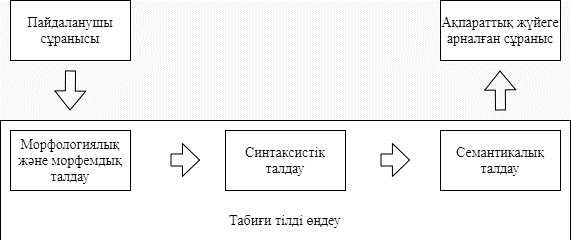
\includegraphics[width=0.8\textwidth]{assets/142}
	\caption*{\bfseries 1 -- сурет. Семантика негізінде табиғи тілдегі сұранысты өңдеу
  әдісінің схемасы}
\end{figure}

\begin{multicols}{2}

Семантикаға негізделген табиғи тілдің сұранысын өңдеу әдісінің схемасы -
табиғи тілдегі қолданушылардың сұраныстарын олардың мағыналық мазмұнын
ескере отырып түсінуге арналған кешенді тәсіл. Бұл әдіс сөйлемнің
грамматикалық құрылымын ғана емес, оның семантикасын, яғни сөздердің
мағыналары мен байланыстарын талдауға негізделген.

Сұранысты өңдеу процесінің басында лексикалық талдау жүргізіледі, оның
барысында мәтін жеке лексемаларға немесе сөздерге бөлінеді. Содан кейін
морфологиялық талдау жүргізіледі, оның нәтижесінде әрбір лексемаға
өзіндік морфологиялық форма беріледі, бұл олардың сөйлеу бөлігін және
грамматикалық сипаттамаларын анықтауға мүмкіндік береді.

Келесі кезекте синтаксистік талдау жүргізіледі, оның барысында сөйлемнің
құрылымы мен оның сөздер арасындағы синтаксистік тәуелділіктері
анықталады. Бұл сұраныстың негізгі құрамдас бөліктерін және олардың
өзара байланысын түсінуге мүмкіндік береді. Бұл ретте сұраныс
контекстіндегі сөздер мен сөз тіркестерінің мағынасы мен мағынасын
анықтауға бағытталған семантикалық талдау орын алады {[}15{]}.

Сұрау мағынасын және оның білім қорымен немесе контекстпен байланысын
тереңірек түсіну үшін машиналық оқыту әдістері мен әдістерін және
жасанды интеллектті қолдануды қамтитын семантикалық өңдеу жүргізіледі.
Бұл семантикалық модельдерді құруды, сөздердің векторлық бейнелерін және
семантикалық графиктерді немесе онтологияларды пайдалануды қамтуы
мүмкін.

Ақырында, талдау мен өңдеудің барлық кезеңдерінен кейін жауап жасалады
немесе сұраныстың түсінілген мағынасына сәйкес тиісті әрекеттер
орындалады. Бұл ақпарат үшін дерекқорды іздеуді, қолданбаларда немесе
жүйелерде операцияларды орындауды немесе пайдаланушы сұрауына табиғи
тілде жауап жасауды қамтуы мүмкін.

Іздеу сұранысын өңдеу логикасындағы негізгі диаграммалар мен
диаграммалар тиімді ақпаратты іздеу жүйелерін жобалаудың негізгі
құралдары болып табылады. Олар сұранысты өңдеу процесін
визуализациялауға және іздеу жүйелерінің логикасын түсінуге көмектеседі.
Негізгі схемалардың бірі сұранысты талдау, сәйкес деректерді іздеу және
нәтижелерді пайдаланушыға ұсыну кезеңдерін қамтитын сұранысты өңдеу
схемасы болып табылады {[}16{]}. Тағы бір маңызды схема - оңай қол
жеткізу және іздеу үшін деректерді ұйымдастыру жолдарын анықтайтын
индекстеу схемасы. Мәліметтер ағынының диаграммалары мен күй
диаграммалары сұранысты өңдеу процесін және жүйе құрамдастарының өзара
әрекетін көрсету үшін де қолданылады. Бұл диаграммалар мен диаграммалар
бірге іздеу жүйелерінің қалай жұмыс істейтіні туралы түсінік береді және
әзірлеушілерге олардың өнімділігі мен функционалдығын оңтайландыруға
көмектеседі (2-сурет).

Ақпаратты іздеу сұрауының реттілігі диаграммасы ақпаратты іздеу сұрауы
кезінде орын алатын әрекеттер тізбегін көрсетеді. Әдетте пайдаланушының
қолданба немесе веб-сайт интерфейсі арқылы сұрауды бастауымен басталады.
\end{multicols}


\begin{figure}[H]
	\centering
	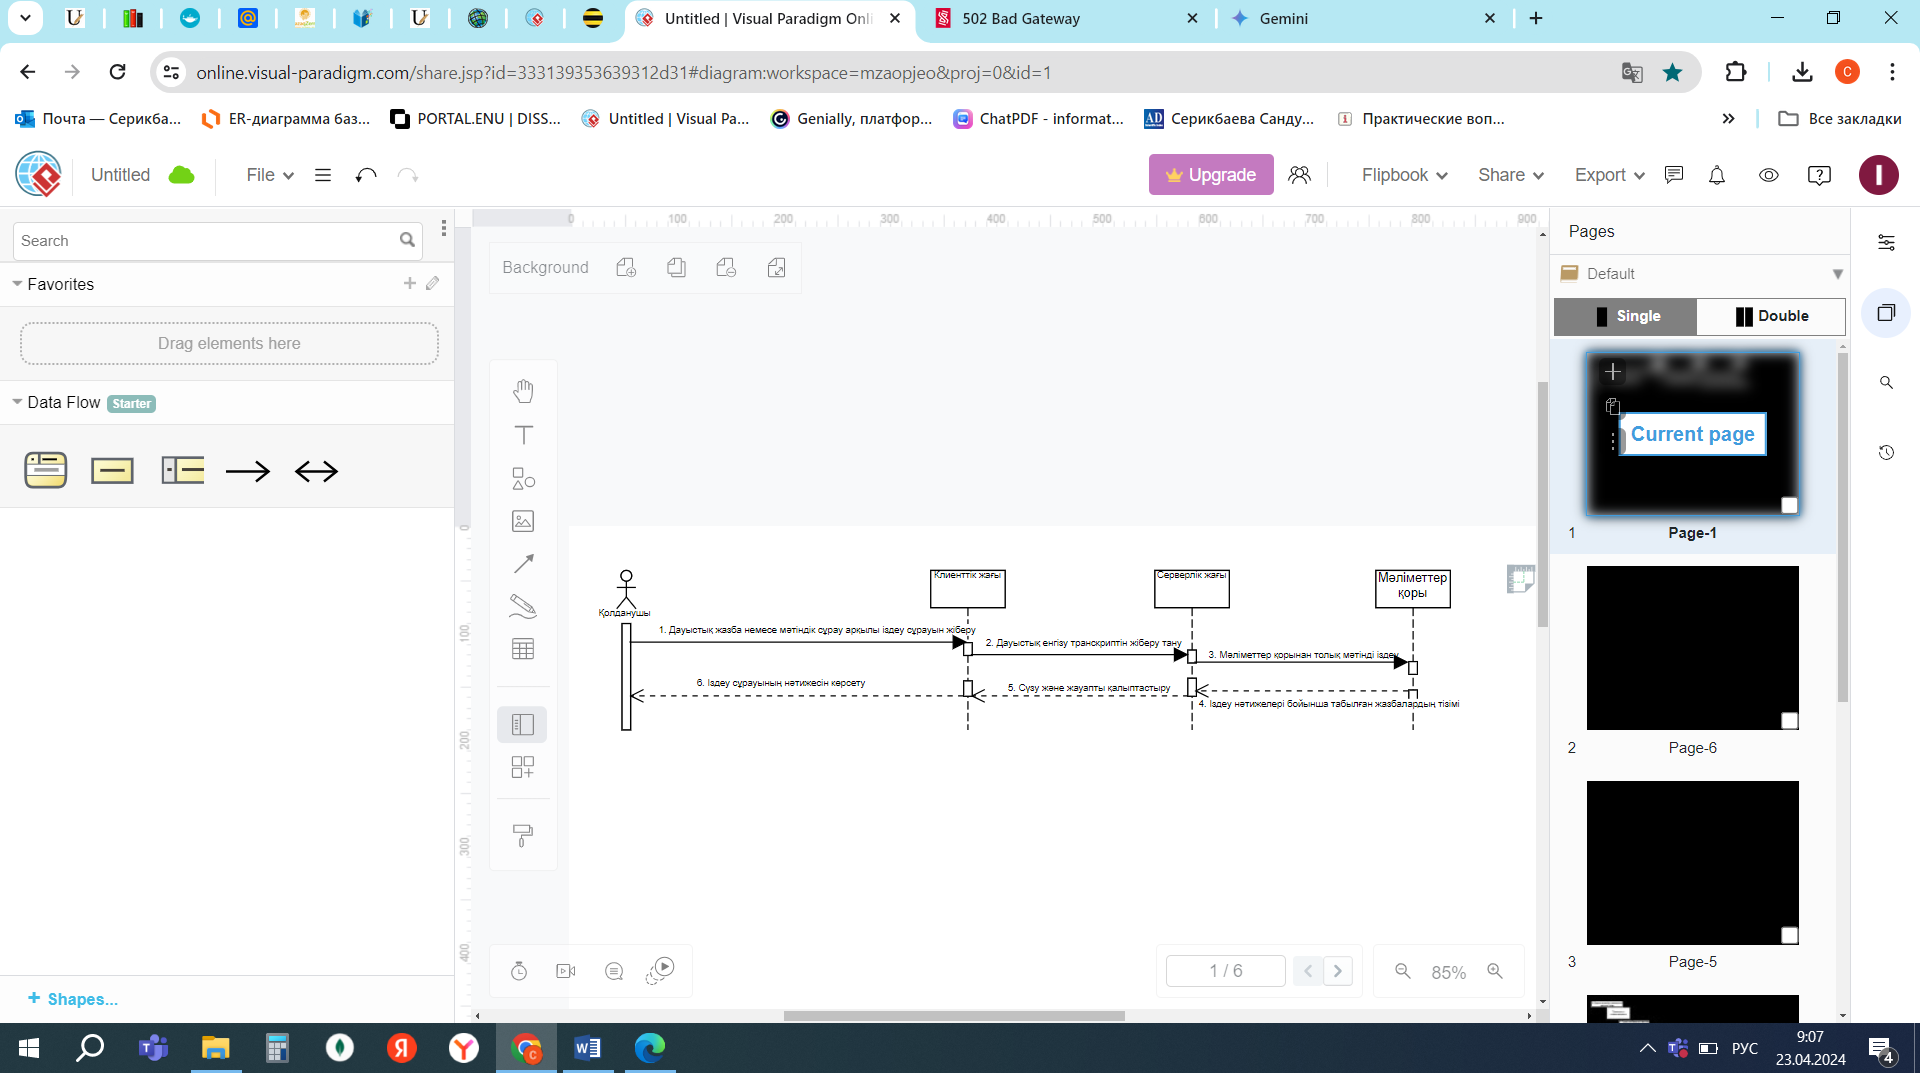
\includegraphics[width=0.9\textwidth]{assets/143}
	\caption*{\bfseries 2 -- сурет. Ақпаратты іздеу сұранысын өңдеуге арналған реттілік
  диаграммасы}
\end{figure}


\begin{multicols}{2}
Содан кейін жүйе бұл сұрауды алады және сұранысты сәйкес іздеу жүйесіне
немесе дерекқорға жіберу арқылы іздеу процесін бастайды. Осыдан кейін
іздеу жүйесі сұрауды талдайды, сәйкес деректерді таңдайды және оны
пайдаланушыға көрсету үшін жүйеге қайтарады. Содан кейін жүйе алынған
нәтижелерді пайдаланушы ақпаратты көре және талдай алатын интерфейс
арқылы пайдаланушыға көрсетеді. Соңында, пайдаланушы сұрауды нақтылау
немесе қосымша зерттеу үшін нақты нәтижені таңдау сияқты берілген
нәтижелерге негізделген қосымша әрекеттерді жасай алады.

Қолданба интеграциясы - алынған ақпаратты қолданба ішінде шешім қабылдау
немесе Пайдаланушымен өзара әрекеттесу үшін пайдалануға болады. Мысалы,
жүйе пайдаланушы-ның сұрағына жауап бере алады, мәтінді іздей алады
немесе мәтіндік хабарламаның көңіл-күйін талдай алады (3-сурет).
\end{multicols}


\begin{figure}[H]
	\centering
	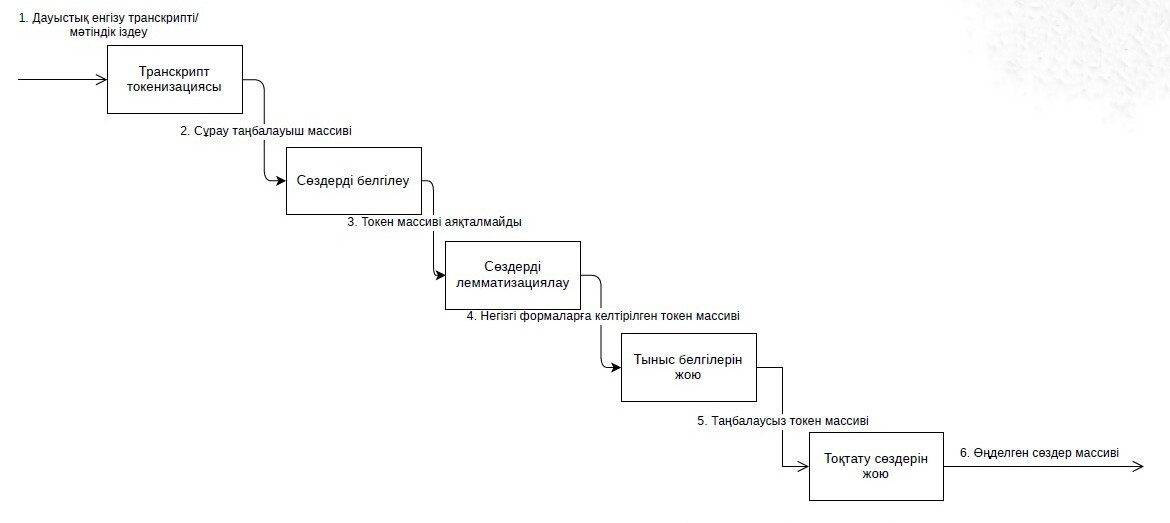
\includegraphics[width=0.9\textwidth]{assets/144}
	\caption*{\bfseries 3 -- сурет. Табиғи тілді өңдеу схемасы}
\end{figure}



\begin{multicols}{2}
Табиғи тілді өңдеу коды:
\end{multicols}

\begin{lstlisting}

  doc = nlp(transcript)
  lemmatized_stemmed_text = [stemmer.stem(token.lemma_.lower()) for token in doc if token.is_alpha and not token.is_stop]
  
\end{lstlisting}



\begin{multicols}{2}
Ақпарат үшін дерекқорды іздеу және клиентке жауап беру туралы сөз
болғанда, тиімді және дәл нәтиже алу үшін белгілі бір қадамдарды орындау
маңызды. Ең алдымен, іздеу критерийлері мен сұраныстың негізгі
параметрлерін анықтау қажет. Бұл нақты іздеу үшін қажетті кілт сөздерді,
күндерді, деректер түрлерін немесе басқа сипаттарды қамтуы мүмкін.

Шарттар анықталғаннан кейін дерекқорды сәйкес құралдар немесе сұрау тілі
арқылы іздеу керек. Дұрыс сұрау синтаксисін және іздеу үшін кестелер мен
өрістерді дұрыс таңдауды ескеру маңызды. Сұрау орындалғаннан кейін
дерекқор сәйкес нәтижелерді қайтарады, содан кейін оларды өңдеу
керек.Алынған деректерді өңдеу клиенттің немесе соңғы пайдаланушының
талаптарына сәйкес ақпаратты талдауды және сүзуді қамтиды. Бұл
сұрыптауды, топтастыруды, есептеулерді және қажетті жауапқа жету үшін
басқа деректерді өңдеуді қамтуы мүмкін. Деректерді өңдегеннен кейін
жауап құрылады, ол құрылымдалған және клиент үшін түсінікті болуы керек.

Маңызды қадам клиентке оны бермес бұрын алынған жауаптың дұрыстығы мен
толықтығын тексеру болып табылады. Бұл деректердің дұрыстығын және
жауаптың көрсетілген критерийлер мен талаптарға сәйкестігін тексеруді
қамтиды. Қажет болған жағдайда ақпаратты нақтылау үшін қосымша
тексерулер мен талдаулар жүргізілуі мүмкін.

Тексеруден кейін жауап клиентке беруге дайын. Бұл мәтіндік хабарлама,
есеп, кесте немесе клиентке қолдануға ыңғайлы басқа пішім түрінде болуы
мүмкін. Ұсынылған жауаптың клиенттің үмітіне сай болуын және оның
сұрауын толық қанағаттандыруын қамтамасыз ету маңызды.

Тиімді іздеуді және клиентке жауап беруді қамтамасыз ету үшін
дерекқордың жаңартылып, жаңартылып тұруын қамтамасыз ету де маңызды. Бұл
нақты іздеу нәтижелерін қамтамасыз ету үшін деректерді үнемі жаңартуды,
жаңа жазбаларды қосуды және ескірген деректерді жоюды қамтиды.

Сонымен қатар, деректердің қауіпсіздігін қамтамасыз ету және деректер
базасына қол жеткізу ережелерін сақтау қажет. Бұған пайдаланушылар үшін
сәйкес кіру құқықтарын орнату және рұқсатсыз кіруді немесе деректерге
өзгертулерді болдырмау үшін деректер әрекетін бақылау кіреді.

Жалпы алғанда, мәліметтер базасын тиімді іздеу және клиентке жауап беру
үшін іздеу критерийлерін анықтау, сұранысты орындау, деректерді өңдеу,
жауаптың дұрыстығын тексеру және оны клиентке ұсыну сияқты жүйелі тәсіл
қажет. Осы қадамдарды орындау ақпараттың клиенттерге дәл және уақтылы
берілуін қамтамасыз етуге көмектеседі (4-сурет).

1. Өңделген таңбалауыштардың массиві табиғи тілде өңдеуден кейін келеді.
Массив толық мәтінді іздеу арқылы дерекқорды іздеуге жіберіледі.

\emph{search\_results = collection.find( \{
\textquotesingle\$text\textquotesingle:
\{\textquotesingle\$search\textquotesingle: \textquotesingle{}
\textquotesingle.join(lemmatized\_stemmed\_text)\} \},
\{\textquotesingle score\textquotesingle:
\{\textquotesingle\$meta\textquotesingle:
\textquotesingle textScore\textquotesingle\},
\textquotesingle workTopic\textquotesingle: 1, "жұмыс атауы":1,\})}

2. Толық мәтінді іздеу нәтижелері курсор ретінде қайтарылады.
Деректермен жұмыс істеудің ыңғайлы нұсқасы үшін түрлендіру әрбір нысан
әрбір жазба туралы деректерді сақтайтын нысандар массивіне жасалады.

\emph{search\_results\_list =
list(search\_results.sort({[}(\textquotesingle score\textquotesingle,
pymongo.DESCENDING){]}))}

3. Іздеу нәтижелері дәл болу үшін табылған объектілерді сүзгілеу
жүргізіледі. Ол үшін жұмыс атауы және жұмыс тақырыбы өрістерін өңдеу
табиғи тілде орындалады.

\emph{for result in search\_results\_list: work\_topic =
result.get(\textquotesingle workTopic\textquotesingle,
\textquotesingle\textquotesingle) \# Получаем значение поля workTopic
work\_name = result.get(\textquotesingle workName\textquotesingle,
\textquotesingle\textquotesingle) \# Получаем значение поля workName \#
Применяем стемминг, лемматизацию и приведение к нижнему регистру
lemmatized\_stemmed\_topic = {[}stemmer.stem(token.lemma\_.lower()) for
token in nlp(work\_topic) if token.is\_alpha and not token.is\_stop{]}
lemmatized\_stemmed\_name = {[}stemmer.stem(token.lemma\_.lower()) for
token in nlp(work\_name) if token.is\_alpha and not token.is\_stop{]}}


\end{multicols}
 

\begin{figure}[H]
	\centering
	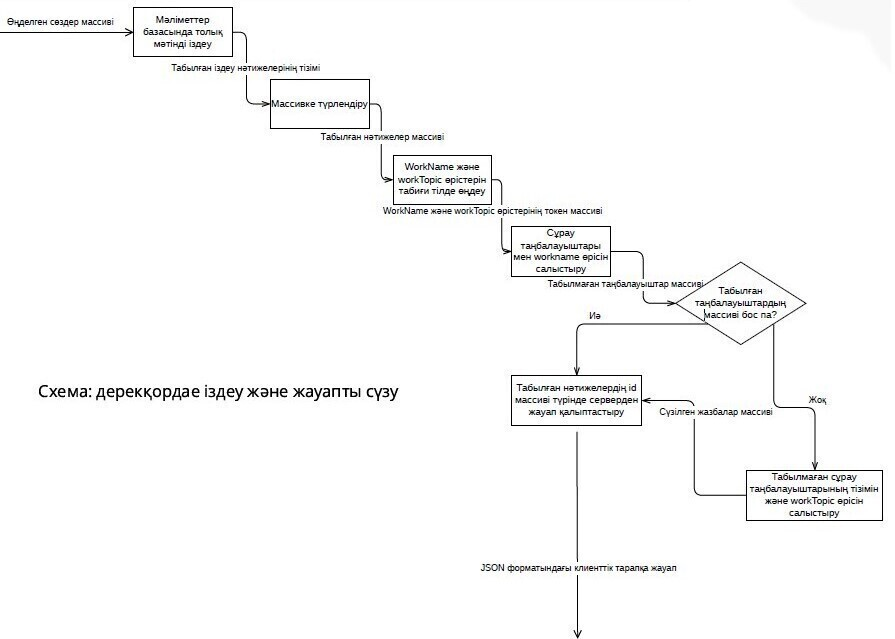
\includegraphics[width=1\textwidth]{assets/145}
	\caption*{\bfseries 4 -- сурет. Деректер қорынан ақпаратты іздеу және клиентке жауап
  беру схемасы}
\end{figure}

\begin{multicols}{2}
4. Өрістерді табиғи тілде өңдегеннен кейін пайдаланушы сұрауының
таңбалауыштары мен жұмыс атауы өрісінің таңбалауыштары салыстырылады.
Табылмаған таңбалауыштар бөлек массивке жазылады.

\emph{if all(word in lemmatized\_stemmed\_name for word in
lemmatized\_stemmed\_text): filtered\_results.\\append(result)
print("result", result) else: \# Определение ненайденных слов
missing\_words = {[}word for word in lemmatized\_stemmed\_text if word
not in lemmatized\_stemmed\_name{]}}

5.Егер табылмаған таңбалауыштардың массиві бос болса, жауапты клиентке
жіберу үшін табылған нәтижелерден жазба идентификаторларының жиымы
жасалады.

6. Егер табылмаған таңбалауыштардың массиві бос болмаса, кеңейтілген
тексеру үшін сұрау таңбалауыштары мен мақаланың аннотация өрістері
салыстырылады. Егер аннотация өрісіндегі барлық белгілер массивте болса,
онда идентификаторды массивке жазамыз және клиентке жауап JSON пішімі
түрінде жасалады.

\emph{if all(word in lemmatized\_stemmed\_topic for word in
missing\_words): filtered\_results.append(result) print("result",
result)}

{\bfseries Нәтижелер мен талдау.} Платформа-пайдаланушыларға белгілі бір
мүмкіндіктерді немесе қызметтерді ұсынатын сандық құрал немесе онлайн
қызмет. Әдетте платформалар белгілі бір тапсырмаларды орындау немесе
пайдаланушылардың белгілі бір қажеттіліктерін қанағаттандыру үшін
жасалады. Олар әлеуметтік желілермен, электрондық коммерциямен,
біліммен, ойын-сауықпен, жобаларды басқарумен және басқа да көптеген
салалармен байланысты болуы мүмкін.

Пайдаланушыларды платформаны пайдалануға тарту үшін жасалған мазмұн оның
сәттілігінде маңызды рөл атқарады. Бұл мазмұн әртүрлі болуы мүмкін және
мақсатты аудиторияны қызықтыратын және қызықтыратын ақпараттық
материалдарды, оқу ресурстарын, интерактивті элементтерді, және басқа
форматтарды қамтуы мүмкін {[}17{]}.

Пайдаланушыларды платформаға тартуға бағытталған мазмұнның негізгі
міндеті-оның құндылығы мен артықшылықтарын көрсету және пайдаланушыларды
әрекетке шақыру. Ол үшін мазмұн мақсатты аудиторияның мүдделері мен
қажеттіліктерін ескере отырып, мазмұнды, тартымды және мақсатты болуы
керек.

Мұндай мазмұнның мысалдары платформаның негізгі мүмкіндіктері мен
артықшылықтарын көрсететін жарнамалық роликтер, пайдаланушы-лардың
шолулары мен шолулары, хэштегтер мен шығармашылық мазмұнды қолданатын
әлеуметтік медиа жазбалары және викториналар, сауалнамалар немесе
конкурстар сияқты интерактивті элементтер болуы мүмкін.

Пайдаланушыларды платформаны пайдалануға тарту үшін мазмұнды құрудың
маңызды сәттері-бұл жарқын дизайн, платформаның негізгі мүмкіндіктерін
түсінікті және тартымды сипаттау, сонымен қатар оны бәсекелестер
арасында ең жақсы таңдау жасайтын ерекше артықшылықтарға баса назар
аудару (5 --сурет) .

Мазмұнды олардың үміттері мен қажеттілікте-ріне бейімдеу үшін
пайдаланушылардың пікірлері мен пікірлерін ескеру маңызды. Мазмұнды
үнемі жаңартып отыру және әртүрлі форматтағы эксперименттер платформаға
деген қызығушылықты сақтауға және жаңа пайдаланушыларды тартуға
көмектеседі.
\end{multicols}



\begin{figure}[H]
	\centering
	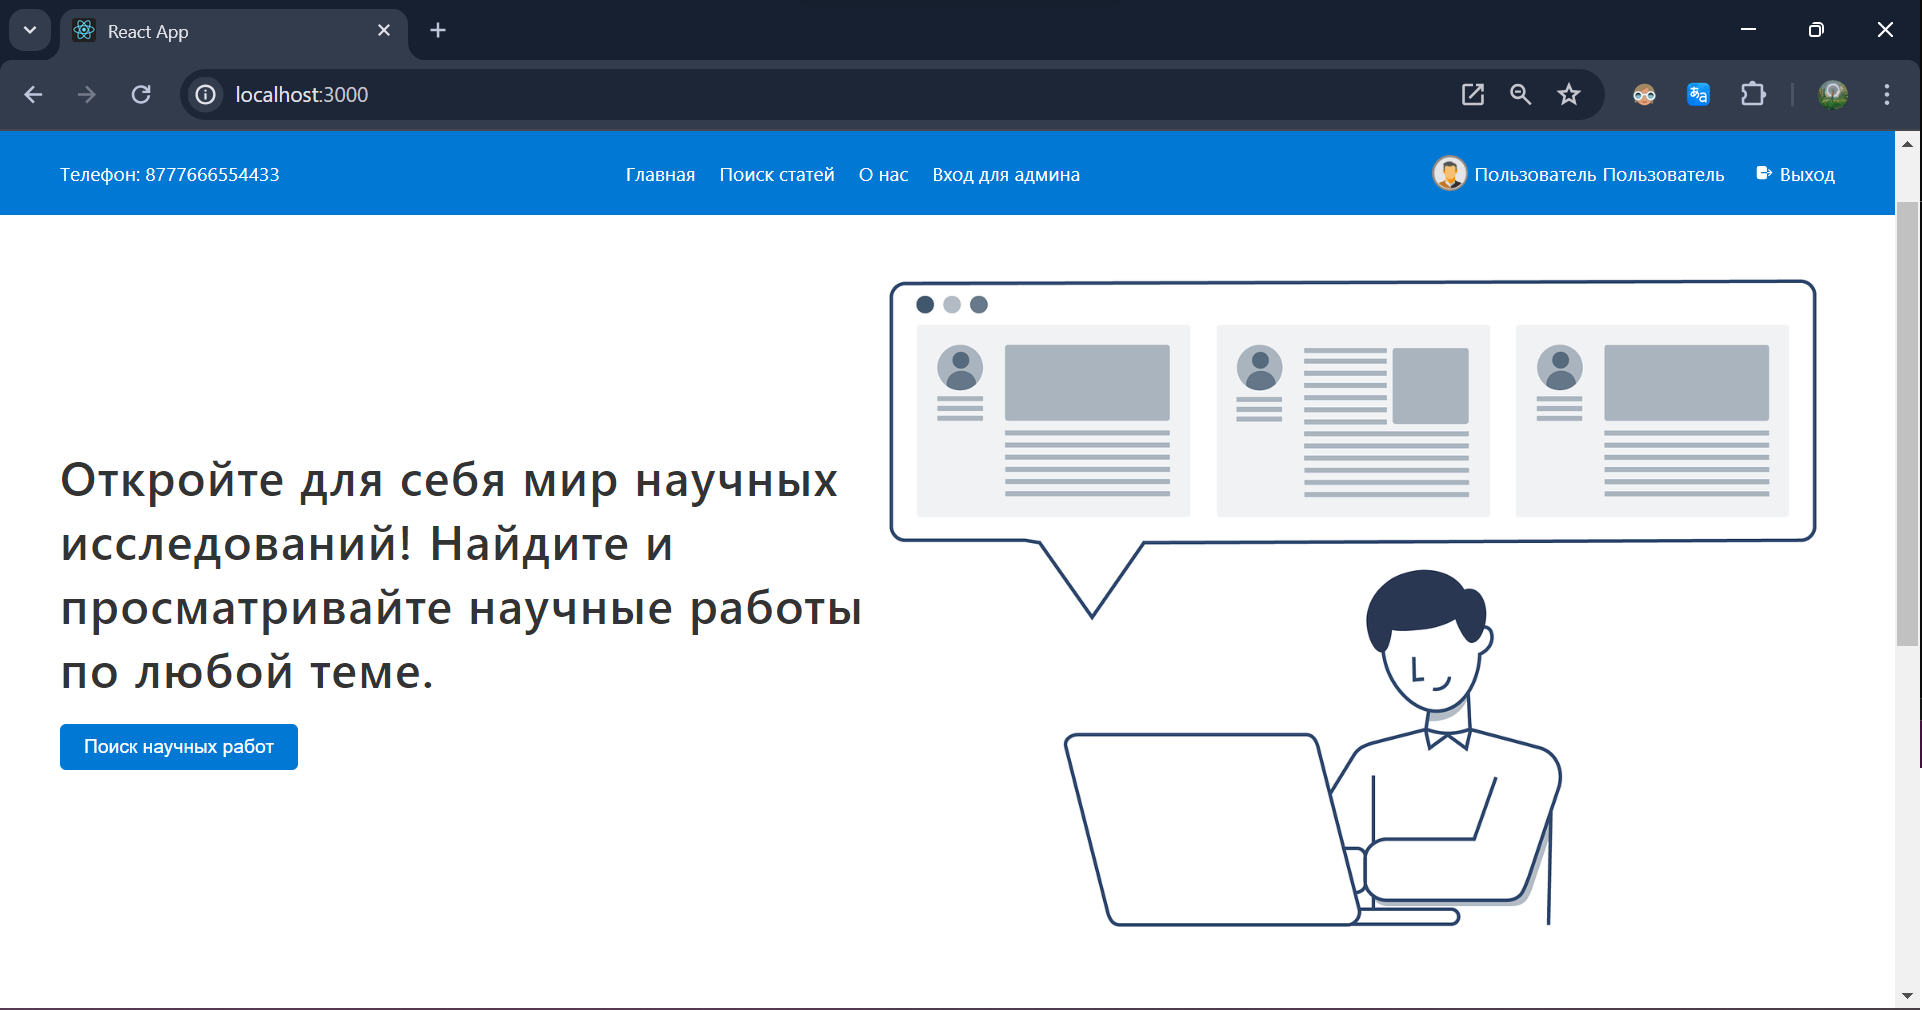
\includegraphics[width=0.8\textwidth]{assets/146}
	\caption*{\bfseries 5 -- сурет. Табиғи тілді қолдана отырып әзірленген интерфейстің
  басты беті}
\end{figure}

\begin{multicols}{2}

{\bfseries Қорытынды.} Пайдаланушы интерфейстерін-дегі табиғи тіл
концепциясын, сондай-ақ оны жобалаудың негізгі принциптері мен әдістерін
зерттеу қазіргі заманғы технологиялардың дамуындағы маңызды кезеңді
білдіреді. Табиғи тілде пайдаланушы интерфейстерін құру саласындағы
қолданыстағы әдістер мен технологияларға шолу осы саланың қазіргі
жағдайы мен даму бағыттарын бағалауға мүмкіндік береді. Мәтінді өңдеу
тәсілдерін, машиналық оқытуды пайдалануды және жасанды интеллект
интеграциясын қоса алғанда, табиғи тілдегі пайдаланушы интерфейстерін
құру әдістері пайдаланушы тәжірибесін және адам мен компьютер арасындағы
тиімді қарым-қатынасты жақсарту үшін кең мүмкіндіктер береді. Мұндай
интерфейстерді құрудың практикалық аспектілеріне сөйлеуді тану
технологияларын пайдалану және оларды әртүрлі қолданбалар мен жүйелерге
біріктіру кіреді, бұл пайдаланушылар үшін ақпараттың ыңғайлылығы мен
қолжетімділігін жақсартуға көмектеседі. Осылайша, табиғи тілдегі
пайдаланушы интерфейстерін одан әрі дамыту және зерттеу адамның
технологиямен өзара әрекеттесуін айтарлықтай жақсартуға және
пайдаланушылардың кең ауқымы үшін анағұрлым интуитивті және тиімді
интерфейстерді құруға мүмкіндік береді.
\end{multicols}


\begin{center}
  {\bfseries Әдебиеттер}
  \end{center}

\begin{noparindent}

\begin{enumerate}
\def\labelenumi{\arabic{enumi}.}
\item
  Елисеева О.Е. Естественно-языковой интерфейс интеллектуальных систем:
  учебное пособие. \\-Минск: БГУИР, 2009.- 151 с. ISBN 978-985-488-323-6
\item
  Ермаков А. Е., Киселев С. Л., Плешко В. В. Поиск фактов в тексте
  естественного языка на основе сетевых описаний // Компьютерная
  лингвистика и интеллектуальные технологии: труды Между-народной
  конференции Диалог. -- 2004. -- С. 282-285.
\item
  Жигалов В.А. Технология построения естественно-языковых интерфейсов к
  структурированным источникам данных: Автореф. дис. \ldots{} кан. тех.
  наук // Москва, 2000 -- 173 с.
\item
  Житко В.А. Пользовательский интерфейс интеллектуальных
  вопросно-ответных системах // Кибер-нетика и программирование. - 2012.
  - № 1. - С.23-30. DOI: 10.7256/2306-4196.2012.1.13862
\item
  Житко В. А. и др. Семантическая технология компонентного
  проектирования естественно-\\языкового интерфейса интеллектуальных
  вопросно-ответных систем. // Труды Международной \\научно-технической
  конференции Open Semantic Technology for Intelligent Sysкtems (OSTIS)
  2011 - 2011.- С. 395-408.
\item
  Крайванова В. А. Модель естественно-языкового интерфейса для систем
  управления сложными техническими объектами и оценка эффективности
  алгоритмов на ее основе // Управление большими системами: сборник
  трудов. -- 2009. -- №. 26 -- С. 158-177.
\item
  Кузнецов Б. А. и др. Обработка запросов на естественном языке новое
  качество поиска в БД ВИН\\ИТИ // НТИ. Серия 2. -- 2001. -- №. 11. -- С.
  31.
\item
  Кузнецова А.И., Ефремова Т.Ф. Словарь морфем русского языка. -- М.
  Русский язык, 1986.-1136 с.
\item
  Николаева И.С., Митренина О.В., Ландо Т.М. Прикладная и компьютерная
  лингвистика // М.: URSS. -- 2016 -- 315 c. ISBN 978-5-9710-3472-8
\item
  Осипов Г. С. и др. Проблемы обеспечения точности и полноты поиска:
  Пути решения в интеллекту-альной метапоисковой системе "Сириус" //
  Труды международной конференции Диалог. -- 2005. -- С. 390-395.
\item
  Посевкин Р.В. Применение семантической модели базы данных при
  реализации естественно-\\языкового пользовательского интерфейса //
  Научно-технический вестник информационных техно-логий, механики и
  оптики.- 2018.-Т. 18(2).-С. 262--267.
  D 10.17586/2226-1494-2018-18-2-262-267
\item
  Посевкин Р.В. Метод автоматизированного формирования семантической
  модели базы данных диалоговой системы // Программные продукты и
  системы.- 2018. -№ 2. -С. 291--294. DOI 10.15827/\\0236-235X.122.291-294
\item
  Посевкин Р.В. Обработка естественного языка в процессе разработки
  пользовательского интерфейса // Сборник научных трудов III
  Международной научной конференции «Информационные техноло-гии в науке,
  управлении, социальной сфере и медицине». -2016.- С. 471- 472. ISBN
  978-5-4387-0672-4
\item
  Посевкин Р.В., Бессмертный И.А. Естественно-языковой пользовательский
  интерфейс диалоговой системы // Программные продукты и системы. -
  2016.- № 3- С.5--9. DOI 10.15827/0236-235X.115.005-009
\item
  Правиков А. А. Разработка и применение метода формализации
  проектирования рекомендательных систем с естественно-языковым
  интерфейсом: дис\ldots канд. технических наук. -Москва, 2011. - 160 с.
\item
  Правиков А.А., Фомичев В.А. Разработка рекомендательной системы с
  естественно-языковым интер-фейсом на основе математических моделей
  семантических объектов // Бизнес-информатика. - 2010. - № 4. - С. 3-8.
\item
  Селезнев К. Обработка текстов на естественном языке //Открытые
  системы. -- 2003. -- Т. 12. \\{[}Электронный ресурс{]}. -- URL:
  https://www.osp.ru/os/2003/12/183694/
\end{enumerate}
\end{noparindent}


\begin{center}
  {\bfseries References}
  \end{center}


\begin{noparindent}
\begin{enumerate}
\def\labelenumi{\arabic{enumi}.}
\setcounter{enumi}{17}
\item
  Eliseeva O.E. Estestvenno-yazykovoi interfeis
  intellektual\textquotesingle nykh sistem: uchebnoe posobie. -- Minsk:
  \\BGUIR, 2009. -- 151 s. ISBN 978-985-488-323-6
\end{enumerate}

\begin{enumerate}
\def\labelenumi{\arabic{enumi}.}
\item
  {[}in Russian{]}
\item
  Ermakov A. E., Kiselev S. L., Pleshko V. V. Poisk faktov v tekste
  estestvennogo yazyka na osnove setevykh opisanii //
  Komp\textquotesingle yuternaya lingvistika i
  intellektual\textquotesingle nye tekhnologii: trudy Mezhdunarodnoi
  konferentsii Dialog. -- 2004. -- S. 282-285. {[}in Russian{]}
\item
  Zhigalov V.A. Tekhnologiya postroeniya estestvenno-yazykovykh
  interfeisov k strukturirovannym istoch-nikam dannykh: Avtoref. dis.
  \ldots{} kan. tekh. nauk // Moskva, 2000 -173 s. {[}in Russian{]}
\item
  Zhitko V.A. Pol\textquotesingle zovatel\textquotesingle skii interfeis
  intellektual\textquotesingle nykh voprosno-otvetnykh sistemakh //
  Kibernetika i programmirovanie. - 2012. - № 1. - S.23-30. DOI:
  10.7256/2306-4196.2012.1.13862 {[}in Russian{]}
\item
  Zhitko V. A. i dr. Semanticheskaya tekhnologiya komponentnogo
  proektirovaniya estestvenno-\\yazykovogo interfeisa intellektual\textquotesingle nykh voprosno-otvetnykh sistem. // Trudy
  Mezhdunarodnoi nauchno-tekhnicheskoi konferentsii Open Semantic
  Technology for Intelligent Sysktems (OSTIS) 2011 -- 2011. --- S.
  395-408. {[}in Russian{]}
\item
  Kraivanova V. A. Model\textquotesingle{} estestvenno-yazykovogo
  interfeisa dlya sistem upravleniya slozhnymi tekhniches-kimi ob"ektami
  i otsenka effektivnosti algoritmov na ee osnove // Upravlenie
  bol\textquotesingle shimi sistemami: sbornik trudov. -- 2009. -- №. 26
  -- S. 158-177. {[}in Russian{]}
\item
  Kuznetsov B. A. i dr. Obrabotka zaprosov na estestvennom yazyke novoe
  kachestvo poiska v BD VINITI // NTI. Seriya 2. -- 2001. -- №. 11. --
  S. 31. {[}in Russian{]}
\item
  Kuznetsova A.I., Efremova T.F. Slovar\textquotesingle{} morfem
  russkogo yazyka. -- M. Russkii yazyk, 1986. -- 1136 s. {[}in
  Russian{]}
\item
  Nikolaeva I.S., Mitrenina O.V., Lando T.M. Prikladnaya i
  komp\textquotesingle yuternaya lingvistika // M.: URSS. -- 2016 -- 315
  c. ISBN 978-5-9710-3472-8 {[}in Russian{]}
\item
  Osipov G. S. i dr. Problemy obespecheniya tochnosti i polnoty poiska:
  Puti resheniya v intellektual\textquotesingle noi metapoiskovoi
  sisteme "Sirius" // Trudy mezhdunarodnoi konferentsii Dialog. -- 2005.
  -- S. 390-395. {[}in Russian{]}
\item
  Posevkin R.V. Primenenie semanticheskoi modeli bazy dannykh pri
  realizatsii estestvenno-yazykovogo
  pol\textquotesingle zovatel\textquotesingle skogo interfeisa //
  Nauchno-tekhnicheskii vestnik informatsionnykh tekhnologii, mekhaniki
  i optiki.- 2018.-T. 18( 2) - S. 262-267. DOI 10.17586/2226-1494-2018-18-2-262-267 {[}in Russian{]}

\item
  Posevkin R.V. Metod avtomatizirovannogo formirovaniya semanticheskoi
  modeli bazy dannykh dialogovoi sistemy //\\ Programmnye produkty i
  sistemy.-2018.- № 2.- S.291- 294.
\end{enumerate}

DOI 10.15827/0236-235X.122.291-294 {[}in Russian{]}

\begin{enumerate}
\def\labelenumi{\arabic{enumi}.}
\setcounter{enumi}{12}
\item
  Posevkin R.V. Obrabotka estestvennogo yazyka v protsesse razrabotki
  pol\textquotesingle zovatel\textquotesingle skogo interfeisa //
  Sbornik nauchnykh trudov III Mezhdunarodnoi nauchnoi konferentsii
  «Informatsionnye tekhnologii v nauke, upravlenii,
  sotsial\textquotesingle noi sfere i meditsine».- 2016.- S. 471-472.
  ISBN 978-5-4387-0672-4 {[}in Russian{]}
\item
  Posevkin R.V., Bessmertnyi I.A. Estestvenno-yazykovoi
  pol\textquotesingle zovatel\textquotesingle skii interfeis dialogovoi
  sistemy // Programmnye produkty i sistemy.-2016.-№ 3-S. 5- 9.
\end{enumerate}

DOI 10.15827/0236-235X.115.005-009 {[}in Russian{]}

\begin{enumerate}
\def\labelenumi{\arabic{enumi}.}
\setcounter{enumi}{14}
\item
  Pravikov A. A. Razrabotka i primenenie metoda formalizatsii
  proektirovaniya rekomendatel\textquotesingle nykh sistem s
  estestvenno-yazykovym interfeisom: dis\ldots kand. tekhnicheskikh
  nauk. -Moskva, 2011. - 160 s. \\{[}in Russian{]}
\item
  Pravikov A.A., Fomichev V.A. Razrabotka
  rekomendatel\textquotesingle noi sistemy s estestvenno-yazykovym
  interfeisom na osnove \\matematicheskikh modelei semanticheskikh
  ob"ektov // Biznes-informatika. - 2010. - № 4. S. 3 - 8. {[}in
  Russian{]}
\item
  Seleznev K. Obrabotka tekstov na estestvennom yazyke //Otkrytye
  sistemy. -- 2003. -- T. 12. {[}Elektronnyi resurs{]}. -- URL:
  https://www.osp.ru/os/2003/12/183694/ {[}in Russian{]}
\end{enumerate}

\end{noparindent}


\emph{{\bfseries Авторлар туралы мәлімет}}


\begin{noparindent}

Танирбергенов Адилбек Жуматаевич -- Л.Н.Гумилев атындағы Еуразия ұлттық
университетінің алгеб-ра және геометрия кафедрасының доцент м.а., Астана,
Қазақстан. E-mail: t.adilbek@mail.ru;

Серикбаева Сандугаш Курманбековна -- Л.Н.Гумилев атындағы Еуразия ұлттық
университетінің Ақпараттық жүйелер кафедрасының аға оқытушысы, PhD,
Астана, Қазақстан. \\E-mail: inf\_8585@mail.ru;

Бөбеева Балнұр Уәлиханқызы - магистр, Орталық Азия Инновациялық
Университеті, «Техника және \\ақпараттық технологиялар кафедрасы»,
Шымкент, Қазақстан. E-mail: Coquette0@mail.ru;

Ахметжанова Шынар Егеубаевна - М.Х.Дулати атындағы Тараз өңірлік
университеті, «Ақпараттық жүйелер» кафедрасының доцент, т.ғ.к., Тараз,
Қазақстан. E-mail: she.akhmetzhanova@dulaty.kz;

Абдувалова Айнур Джумабевна- М.Х.Дулати атындағы Тараз өңірлік
университеті, «Ақпараттық жүйелер» кафедрасының доцент м.а., т.ғ.к.,
Тараз, Қазақстан. E-mail: abduvalova\_ad@mail.ru.

\end{noparindent}

\emph{\bfseries Information about the authors}

\begin{noparindent}
Tanirbergenov Adilbek - associate professor of the Department of algebra
and geometry, L.N. Gumilyov Eurasian National University, Astana,
Kazakhstan. E-mail: t.adilbek@mail.ru;

Serikbayeva Sandugash - PhD, Senior Lecturer of the Department of
Information Systems, L.N. Gumilyov Eurasian National University, Astana,
Kazakhstan. E-mail: inf\_8585@mail.ru;

Bobeeva Balnur - master\textquotesingle s degree, Central Asian
Innovation University, Department of Technology and information
technologies, Shymkent, Kazakhstan. E-mail: Coquette0@mail.ru;

Akhmetzhanova Shynar - acting associate professor of the Department
«Information Systems», Taraz regional university named after M. KH.
Dulaty, Taraz, Kazakhstan. E-mail: she.akhmetzhanova@dulaty.kz;

Abduvalova Ainur - acting associate professor of the Department
«Information Systems», Taraz regional university named after M. KH.
Dulaty, Taraz, Kazakhstan. E-mail: abduvalova\_ad@mail.ru
\end{noparindent}
